\section{Approach}
\label{sec:2-step-supervised-method}

\begin{figure}[th]
        \centering
        %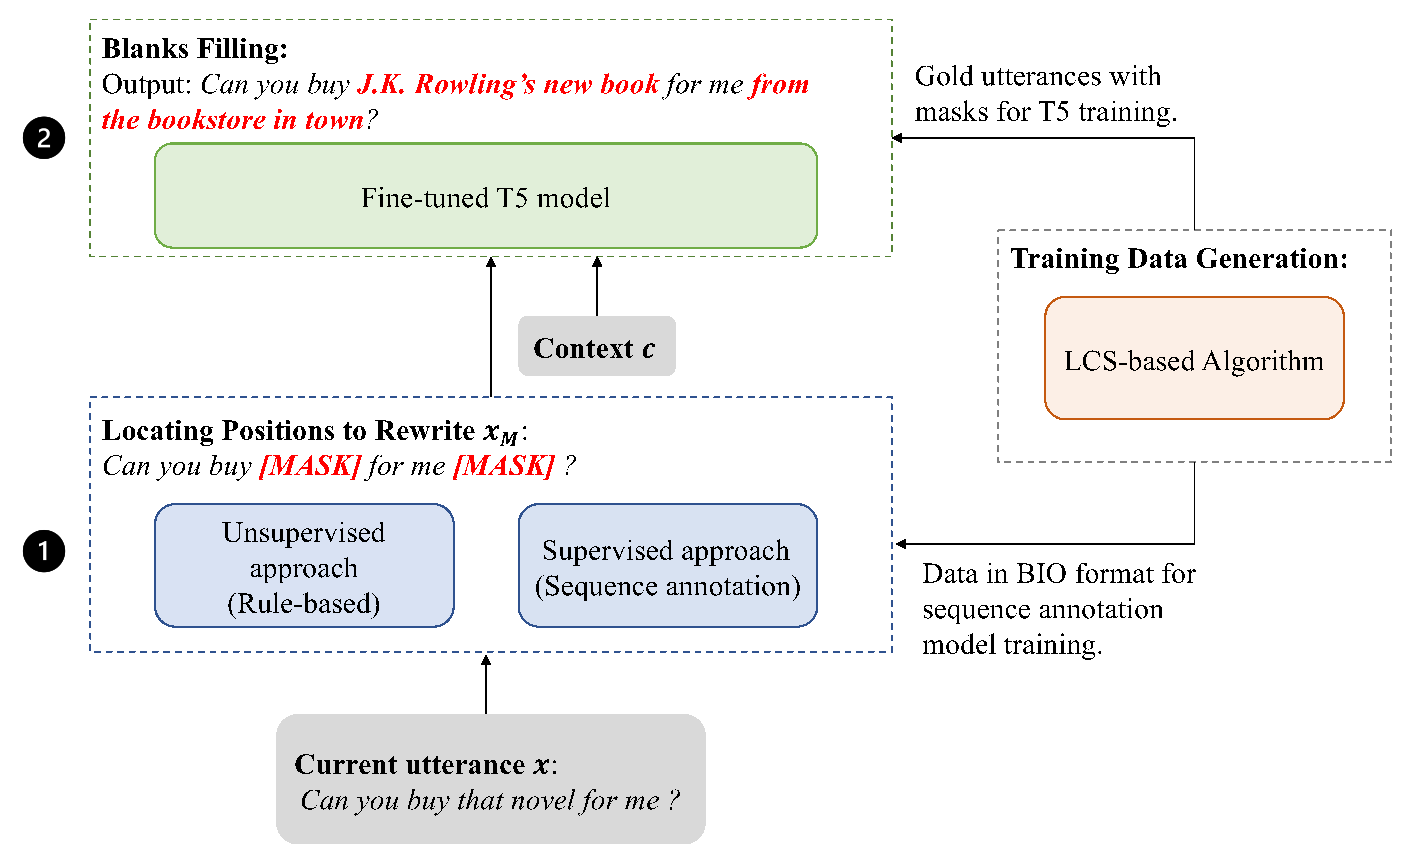
\includegraphics[width=1.7\columnwidth]{framework.eps}
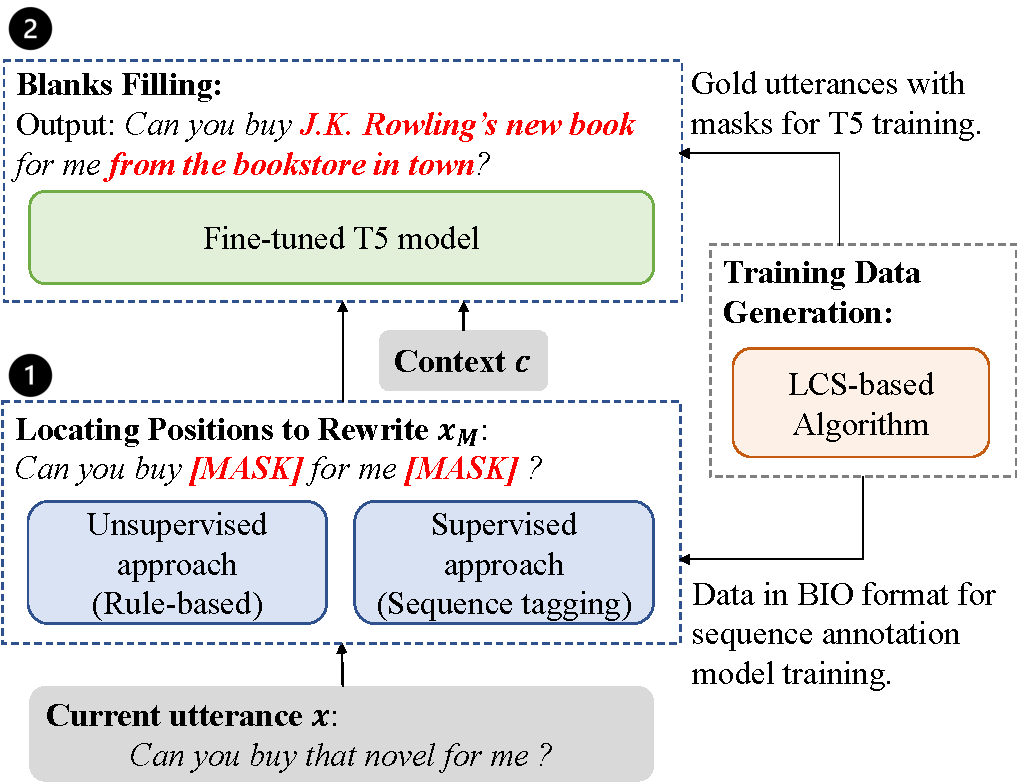
\includegraphics[width=\columnwidth]{fr1-crop.pdf}
        \caption{Our 2-phase rewrite framework.}
% \KZ{This is NOT a framework, more like an example of
%a workflow.}}
        \label{fig:framework}
\end{figure}
%\KZ{Do NOT label your figs and tables as fig1 and fig2. Use something more descriptive.}

Our framework is divided into two phases: \textbf{Locating positions to rewrite} and 
\textbf{Filling the blanks}. 
\figref{fig:framework} is a brief schematic of the framework.
Phase 1 can be done either by heuristic rules or by supervision. 
Phase 2 can be done with a seq2seq text generation model. 
We give the details of these phases next.
%Firstly, the input rewriting dataset is preprocessed to generate the training data required by the above two steps. Align the utterance before and after rewriting to get the spans of coreference and ellipsis. This preprocessing can be solved by an algorithm based on the longest common subsequence (LCS) or a greedy algorithm. In practice, the algorithm based on LCS has better effect. Then, using the two groups of data obtained by preprocessing, train the sequence 
%labeling module and the blank filling module respectively. Finally, input the results obtained from the sequence annotation into the blank filling module, output the filled words, and then get the final rewriting utterance.


 









\subsection{Locating Positions to Rewrite}

We designed an unsupervised and a supervised method to locate positions to rewrite. The two methods are described below.


\subsubsection{Unsupervised Rule-based Method}
\label{sec:ruolan-rule}
%Ruolan should write this part, 
%and this part should be 
%moved into ablation test section.
We first implement a rule-based method for the first phase
of our problem, aiming at predicting the blanks automatically.
We looked through thousands of complete utterance examples
in \citet{elgohary-etal-2019-unpack}. 
Based on our observations
and experience,
we define six rules for generating 
two kinds of blanks which are used for 
resolving coreference and ellpisis
in the second phase.
The rules for generating blanks are 
summarized and explained below:

\noindent
\textbf{Personal Pronouns:} We replace all the personal pronouns
(except the first- and second-person pronouns)
 and their 
corresponding possessive pronouns with
[MASK\_r].
This indicates that we will replace these pronouns with
some specific noun phrases at second phase.

\noindent
\textbf{Interrogatives:}
We insert [MASK\_i] after the 
interrogative
if the whole utterance only contains 
interrogatives such as what, how, why, when
and so forth. [MASK\_i] indicates that some additional
text span shall be inserted at this location.

\noindent
\textbf{That, This:}
The use of word like ``this'', ``that'', ``these'' and ``those''
are commonly used in colloquial language,
which becomes a source of ambiguity.
Therefore, we deal with the use of these pronouns in following ways:
\begin{itemize}
\item[-] Not followed by a noun phrase: In this case, we simply replace the word by [MASK\_r].
\item[-] Otherwise: We will insert [MASK\_i] after the noun phrase.
\end{itemize}

\noindent
\textbf{The + Noun Phrase:}
We will insert [MASK\_i] after the noun phrase.

\noindent
\textbf{Other, Another, Else:}
If the utterance contains these words,
it usually indicates that
 there are people/things 
additional to what have been mentioned
before.
Hence,
we add a [MASK\_i] 
at the head of the sentence.

\noindent
\textbf{Before, After:}
%\KZ{rephrase this sentence, don't understand: 
We insert [MASK\_i] after the sentence 
ended with ``before'' or ``after'',
which is considered as an incompletion.
%as the sentence is incompleted.}

%\KZ{If we use the rule-based method to locate the spots to fill,
%what about the training step for phase 2? This is never discussed.
%This section is like only half way done. The next section is
%a method that not only generate data for phase 1 but also phase 2.
%Seems this section and the next are not compatible.}




\subsubsection{Supervised LCS-based Method}
\label{sec:becky-lcs}
%\KZ{I think this subsection should be taken out and put it side-by-side with the previous
%rule-based approach. These two are two different ways of generating data.
%The next two subsections are about how to train the two-phase models using the
%generate data.}
We also design an algorithm based on the Longest Common Subsequence (LCS)
algorithm
%, which has a better effect
.
The sentence to be rewritten \textbf{X} and after rewriting \textbf{Y} are aligned via a sequence labeling model. To obtain the common subsequence, LCS algorithm returns a matrix \textbf{M} which stores the LCS sequence for each step of the calculation. The value of $M_{i,j}$ indicates the actual LCS length of sequences $X[0,i]$ and $Y[0,j]$\footnote{https://en.wikipedia.org/wiki/

Longest\_common\_subsequence\_problem}. 
When we trace back from the max value at the corner, the decreases of length show that the sentences have had a common token.

%Then t
%The modification including 
Coreference and ellipsis towards original sentence is extracted through LCS trace back algorithm, which is further labeled as COR and ELL respectively. Given the tokenized original sentence \textbf{X} and ground truth \textbf{Y} as shown in \figref{fig:lcs}, the rules for labeling are specified as follows:
\begin{itemize}
\item {
%We follow 
The labeling is proceeded from the bottom right to the top left corner of a LCS matrix. If the current tokens in $X_i$ and $Y_j$ are equal, $X_i$ matches part of the LCS and is labeled as O, then we go both up and left (shown in black). If not, we go up or left, depending on which cell has a higher number or lower index $j$, until we find next matched $X_{i’}$ that satisfies $X_{i’}=Y_{j'}$.} 
\item {If traversed path from previously matched token pair to newly match pair is a straight up arrow, it indicates that token(s) in interval
$(Y_{j’},Y_j)$~\footnote{($a$, $b$) means an open interval excl. the endpoints $a$ and $b$.}
is (are) inserted at corresponding position $i’$ in \textbf{X} to complete 
the original sentence. In this case, token $X_{i’}$ is labeled as ELL(shown in orange).}
\item {If two matched pairs in the LCS matrix are joined by paths with corners, interval $(X_{i’},X_i)$ is replaced by $(Y_{j’},Y_j)$ during rewriting. As a result, coreferenced words are labeled as COR(shown in blue).}
\end{itemize}

\begin{figure}[th]
        \centering
        \includegraphics[width=1.0\columnwidth]{lcs.eps}
        \caption{Example of generating sequence labeling data (based on LCS).}
        \label{fig:lcs}
\end{figure}



%\subsubsection{Locating Positions to Rewrite}
%\label{sec:ner-method}

\begin{figure}[th]
        \centering
        \includegraphics[width=1.0\columnwidth]{locate-rewrite.eps}
        \caption{Generate training data in BIO format.}
        \label{fig:locate-rewrite}
\end{figure}

Then, we input the pre-processed training data into the Bert-CRF \citep{DBLP:journals/corr/abs-1909-10649} 
model, 
%thinking of this step
which is considered as a sequence annotation task. 
Using the method described in \secref{sec:becky-lcs}, we obtained the locations of coreferences 
and ellipses of each utterance waiting to be rewritten. As shown in \figref{fig:locate-rewrite}, 
we use the BIO format to annotate the sequence. The starting position of the coreference is 
marked as B-COR (Begin-Coreference), %. The middle and last 
while other positions of the coreference are marked as I-CORs (Inside-Coreference). Ellipsis only appears in the middle of two tokens, so we mark the position of the latter token as B-ELL (Begin-Ellipse), which means that there should be missing words between this token and the previous token, and the subsequent model is required to fill in it.






\subsection{Blanks Filling}
\label{blanks-filling}

\begin{figure}[th]
        \centering
        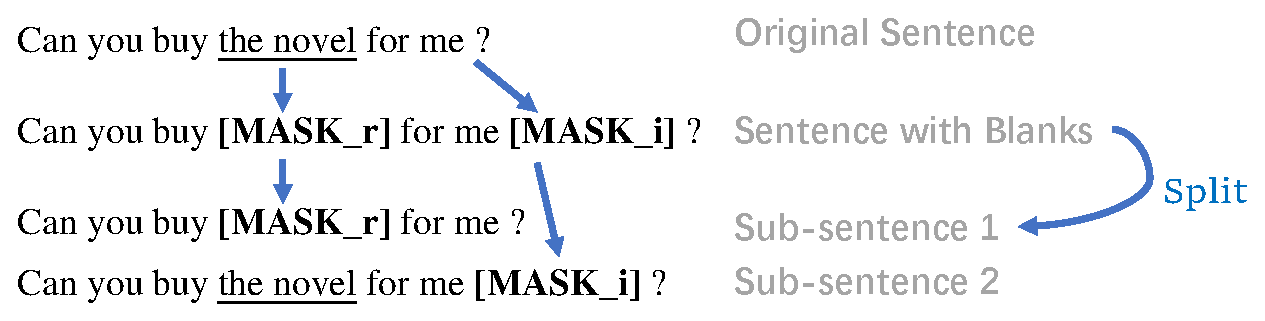
\includegraphics[width=1.0\columnwidth]{add-split.eps}
        \caption{Split the sentence according to the number of blanks in the utterance.}
        \label{fig:add-split}
\end{figure}

\begin{figure}[th]
        \centering
        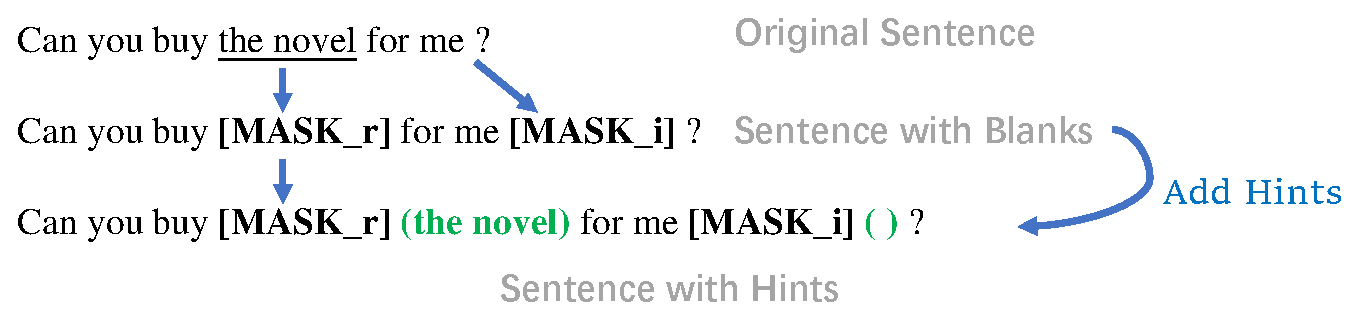
\includegraphics[width=1.0\columnwidth]{add-hint.eps}
        \caption{Add hints to blanks.}
        \label{fig:add-hint}
\end{figure}

We use the T5 model \citep{2020t5} to fill in blanks
%, and use 
with two optimizations: adding hints and splitting the current utterance into sub-sentences. 
%according to the number of blanks. 
The latter can ensure that there is only one blank in the sentence to be filled in the T5 model. The two optimizations are shown in \figref{fig:add-split} and \figref{fig:add-hint}. We transfer the data of each multi-turn dialogue into the format shown in \figref{fig:T5-format}, and fine-tune the T5 model for 20 epochs.

\begin{figure}[th]
        \centering
        \includegraphics[width=1.0\columnwidth]{T5-format.eps}
        \caption{Format of fine-tune data of T5.}
        \label{fig:T5-format}
\end{figure}

After fine-tuning, we take the predicted results of Bert-CRF model in \secref{sec:becky-lcs} as input to get the final blank filled results of T5 model. Finally, the outputs of T5 model are filled back into the blanks of the original sentence to get the rewritten utterance. 
%When the rule-based method in \secref{sec:ruolan-rule} is used, it is similar.
The same is for the rule-based method.
 The blank prediction obtained from it is directly input into the same T5 model (the two optimization methods described in \figref{fig:add-split} and \figref{fig:add-hint} will also be used) to obtain the output of T5.
